\documentclass[border=6pt]{standalone}
\usepackage[T1]{fontenc}
\usepackage[utf8]{inputenc}
\usepackage{mathptmx}
\usepackage{amsmath,amssymb,amsfonts,mathrsfs}
\usepackage[dvipsnames]{xcolor}
\usepackage{tikz}
\usetikzlibrary{calc,positioning,arrows.meta,decorations.pathreplacing,
                decorations.markings,matrix,fit,backgrounds,shapes.misc}
\renewcommand{\sl}{\mathfrak{sl}}
\newcommand{\Uq}{U_q(\sl_2)}
\newcommand{\qint}[1]{[#1]_q}
\newcommand{\Rcheck}{\check{R}}
\definecolor{accent}{RGB}{59,91,146}
\definecolor{accentsoft}{RGB}{155,180,216}
\definecolor{oddsign}{RGB}{138,40,132}
\tikzset{
  strand/.style={line width=1pt, accent!80!black},
  rbox/.style={draw=accent!70!black, fill=accentsoft!55, rounded corners=2pt,
               line width=0.8pt, minimum height=6mm},
  rdot/.style={circle, fill=accent, inner sep=1.6pt},
  knode/.style={circle, draw=accent!70!black, fill=accentsoft!45,
                line width=0.8pt, minimum size=7mm, font=\small},
  kedge/.style={accent!70!black, line width=0.9pt},
  faredge/.style={oddsign!75!black, line width=0.9pt, densely dashed},
  glabel/.style={font=\footnotesize, accent!60!black},
}
\begin{document}
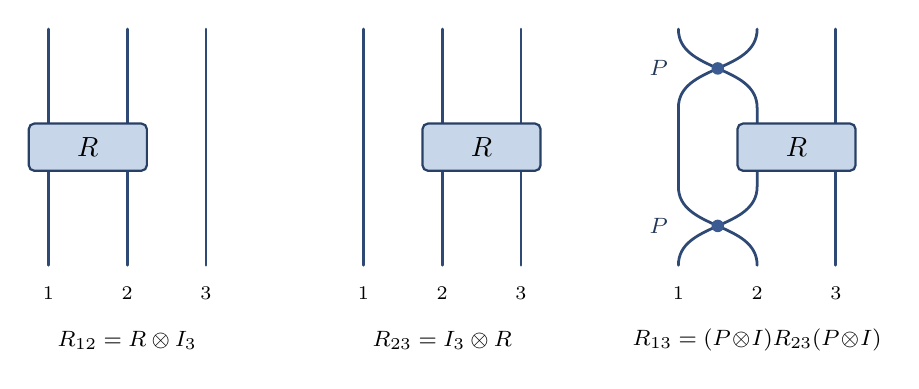
\begin{tikzpicture}[x=1cm,y=1cm,line cap=round]
  % ---- R12 ----
  \begin{scope}
    \draw[strand] (0,0)--(0,3); \draw[strand] (1,0)--(1,3); \draw[strand] (2,0)--(2,3);
    \node[rbox, minimum width=15mm] at (0.5,1.5) {$R$};
    \foreach \k/\x in {1/0,2/1,3/2}{\node[font=\scriptsize] at (\x,-0.35){\k};}
    \node[font=\footnotesize] at (1,-0.95) {$R_{12}=R\otimes I_3$};
  \end{scope}
  % ---- R23 ----
  \begin{scope}[xshift=4cm]
    \draw[strand] (0,0)--(0,3); \draw[strand] (1,0)--(1,3); \draw[strand] (2,0)--(2,3);
    \node[rbox, minimum width=15mm] at (1.5,1.5) {$R$};
    \foreach \k/\x in {1/0,2/1,3/2}{\node[font=\scriptsize] at (\x,-0.35){\k};}
    \node[font=\footnotesize] at (1,-0.95) {$R_{23}=I_3\otimes R$};
  \end{scope}
  % ---- R13 (konjugasyon) ----
  \begin{scope}[xshift=8cm]
    % strand A: 0 -> swap -> pos1 -> swap back -> 0
    \draw[strand] (0,0) to[out=90,in=-90] (1,1) -- (1,2) to[out=90,in=-90] (0,3);
    % strand B: 1 -> 0 -> 1
    \draw[strand] (1,0) to[out=90,in=-90] (0,1) -- (0,2) to[out=90,in=-90] (1,3);
    % strand C: 2 duz
    \draw[strand] (2,0) -- (2,3);
    % P kesisimleri
    \node[rdot] at (0.5,0.5){}; \node[rdot] at (0.5,2.5){};
    \node[glabel] at (-0.25,0.5){$P$}; \node[glabel] at (-0.25,2.5){$P$};
    % R kutusu orta bolgede pos2(=x1) ve pos3(=x2) uzerinde
    \node[rbox, minimum width=15mm] at (1.5,1.5) {$R$};
    \foreach \k/\x in {1/0,2/1,3/2}{\node[font=\scriptsize] at (\x,-0.35){\k};}
    \node[font=\footnotesize] at (1,-0.95) {$R_{13}=(P\!\otimes\! I)R_{23}(P\!\otimes\! I)$};
  \end{scope}
\end{tikzpicture}
\end{document}
